Build systems sometimes referred as build automations, are widely
understood solutions that automates processes related to software
building, the most important of which are in a narrower sense compiling,
packing, testing, or in a broader sense also processes included in
continuous integrations and continuous deployment. The rest of the
chapter will focus mainly on the first meaning of the concept.

\hypertarget{advantages-of-using-build-systems}{%
\section{Advantages of using build
systems}\label{advantages-of-using-build-systems}}

The main reasons of using this type of tools includes:

\begin{itemize}
\item
  time saving and resistance to mistakes
\end{itemize}

The most obvious advantage of automation is time savings. The complexity
of the build processes could be not only excessively time-consuming
while it is manually operated but also leads to numerous mistakes.

\begin{itemize}
\item
  consitiency and portability
\end{itemize}

Depending on the technology stack used in the project, the result may
differ depending on the specific environment. Build system can mitigate
this risk by standardizing some elements of the environment such as
versions of compilers, runtime systems, dependencies and also
compilation parameters or environment variables.

\begin{itemize}
\item
  reproducable builds
\end{itemize}

This feature results from the previous point. Build reproducibility can
be important to maintaining the credibility of open source projects and
in some cases it can may help detect compromised build chains leading to
the next feature.

\begin{itemize}
\item
  security
\end{itemize}

Build system can contribute to increased security by the fact that it
facilitates the separation of the environment in which the application
is developed and in which it is built.

\begin{itemize}
\item
  dependency resolving
\end{itemize}

Depending on the specific system, it can help to varying degrees in
managing dependencies from local resources as well as remote ones.

\begin{itemize}
\item
  better audibility
\end{itemize}

The more descriptive nature of the configuration makes it easier to
identify certain characteristics, mostly related to versions of
environment components or dependencies.

\begin{itemize}
\item
  tasks parallelization
\end{itemize}

Build system can perform multiple tasks in parallel as long as the order
of dependencies is followed.

\hypertarget{overview-of-selected-build-systems}{%
\section{Overview of selected build
systems}\label{overview-of-selected-build-systems}}

This section of the chapter covers some of the building automation
tools. Due to the enormity of the possibilities of each of them, the
analysis is focused on presenting the features that are particularly
important for a given one, and at identifying the differences between
them.

\hypertarget{gnu-make}{%
\subsection{GNU Make}\label{gnu-make}}

The first system described in this chapter is Make, actually its
implementation from the GNU project. Make, as a utility included in the
POSIX standard\cite{MAKEPOSIX}, is a fairly common build system. Its implementations
differ in terms of specific functionalities, but remain largely
compatible. For simplicity, Make is hereinafter referred to as GNU Make.

Make is language-agnostic and is not limited to building only, but can
be easily used to automate any related side tasks. It is facilitated by
the simple syntax of the Makefile file, which define the rules in which
the declared targets should be executed. Makefiles can be human-written
or automatically generated by high-level build systems such as CMake,
GNU Autotools, or Meson. Make comes with an extensive set of tools that
can simplify the manual creation of makefiles.

The basis of makefiles are rules. They have the following syntax.

\begin{verbatim}
target: dependencies
    system command(s)
\end{verbatim}

The example below shows the contents of a simple makefile. The program
built by Make in this case will be called edit, like the first target.
The first target is the default one and will run if you run
\texttt{make} with no additional parameters. A specific target can be
called using \texttt{make\ \textless{}target\textgreater{}}.

\begin{lstlisting}[frame=single, caption={%
  Example of simple MakeFile \cite{MAKEFILE}%
}]
objects = main.o command.o display.o utils.o

edit : $(objects)
        cc -o edit $(objects)
main.o : main.c defs.h
        cc -c main.c
command.o : command.c defs.h command.h
        cc -c command.c
display.o : display.c defs.h buffer.h
        cc -c display.c
utils.o : utils.c defs.h
        cc -c utils.c
clean :
        rm edit $(objects)
\end{lstlisting}

The target can be a file like the listed object files and executable, or
an action like the clean target. If the target is a file, by default
make will check whether the source file has changed since the target
file was created and decide on that basis if it should be rebuilt.
Changing dependencies will also trigger a rebuild for the proper units.

Make's functionality includes:

\begin{itemize}
\item
  echoing
\item
  variables (sometimes referred as macros)
\item
  build in functions like \texttt{prefix}, \texttt{foreach},
  \texttt{eval}, \texttt{shell}
\item
  conditional expressions
\end{itemize}

and many more to make makefiles more convenient when read and written by
users. These features make it very versatile tool.

\hypertarget{ninja}{%
\subsection{Ninja}\label{ninja}}

Ninja is relatively new software. It was created to speed up the
building of very large projects consisting of many thousands of files.
Work on this project started in 2010, when its creator Evan Martin was
working on the Google Chrome browser. The browser code back then
consisted of around 40,000 source files[\cite{NINJACHROME}], which explains the desire to
speed up the application building process.

The syntax of the .ninja files that define the build process is trivial
and is basically limited to rules that allow you to define short names
for complex commands, variables, and expressions thats works just like
in Make. If the target on the left is older than the source on the left,
the target will be rebuilt. Sample ".ninja" file code below.

\begin{lstlisting}[frame=single, caption={%
  Example of simple .ninja file \cite{NINJAFILE}%
}]
cflags = -Wall

rule cc
  command = gcc $cflags -c $in -o $out

build foo.o: cc foo.c
\end{lstlisting}

There are several aspects related to the simplicity of this solution. It
allowed to create a hand-written and very efficient lexer and parser
which sped up significantly the parsing process. Removal of redundant
functionalities not only helped to improve performance, because Ninja do
not have to call additional subroutines to handle these, but even check
whether they have been used as if only the simplest Make expression was
used. It also makes the ".ninja" file for a large project inconvenient to
write manually. Therefore it is assumed that Ninja should be used in
conjunction with another higher level build system such as CMake.

The performance of the Ninja is demonstrated by the benchmark result by
David Röthlisberger\cite{BENCHMARK}.

\begin{quote}
For a project with 1,000 programs built from 10,000 C files and 10,000
header files, there is no significant difference in the duration of a
fresh build. A no-op build takes less than a second with make (0.87s
versus 0.13s with Ninja), probably not enough to really matter for
interactive use.
\end{quote}

\begin{quote}
For a much larger project (10,000 programs, 100,000 C files and 100,000
header files) there is a significant difference in a no-op build: 73s
for Make versus 1.5s for Ninja. Make spends 98\% of that time processing
the 100,000 compiler-generated ``.d'' files that are used for tracking
implicit dependencies on header files.
\end{quote}

\begin{figure}
\centering
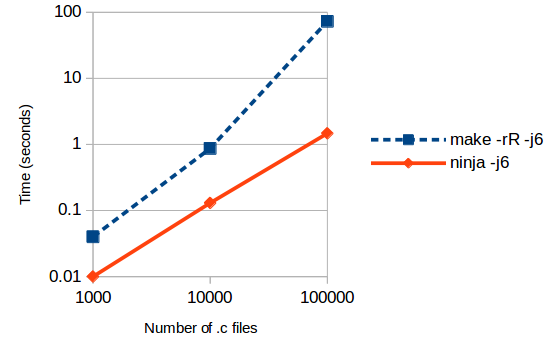
\includegraphics{./no-op-build.png}
\caption{No-op build}
\end{figure}

\hypertarget{maven}{%
\subsection{Maven}\label{maven}}

Maven is significantly different from previous systems. It is intended
for managing Java based projects. Projects are configured by pom.xml
file, which, unlike the previous configuration files, is more
declarative. In addition to meta information, it contains a list of
dependencies, repositories from which the external packages can be
downloaded and a list of plugins with a configuration. The entire system
is based on a plugin mechanism that can be attached from external
sources. Additional configuration or new functionality, e.g.~how to
build a package or how to deploy application, can be added and
configured using plugins. Below is an example pom.xml file.

\begin{lstlisting}[frame=single, caption={%
  Example of simple pom.xml file \cite{POMFILE}%
}]
<project xmlns="http://maven.apache.org/POM/4.0.0" 
xmlns:xsi="http://www.w3.org/2001/XMLSchema-instance"
  xsi:schemaLocation="http://maven.apache.org/POM/4.0.0
  http://maven.apache.org/xsd/maven-4.0.0.xsd">
  <modelVersion>4.0.0</modelVersion>
 
  <groupId>com.mycompany.app</groupId>
  <artifactId>my-app</artifactId>
  <version>1.0-SNAPSHOT</version>
 
  <name>my-app</name>
  <url>http://www.example.com</url>
 
  <properties>
    <project.build.sourceEncoding>UTF-8</project.build.sourceEncoding>
    <maven.compiler.source>1.7</maven.compiler.source>
    <maven.compiler.target>1.7</maven.compiler.target>
  </properties>
 
  <dependencies>
    <dependency>
      <groupId>junit</groupId>
      <artifactId>junit</artifactId>
      <version>4.11</version>
      <scope>test</scope>
    </dependency>
  </dependencies>
 
  <build>
      <plugins>
        <plugin>
          <groupId>org.apache.maven.plugins</groupId>
          <artifactId>maven-compiler-plugin</artifactId>
          <version>3.3</version>
          <configuration>
            <source>1.5</source>
            <target>1.5</target>
          </configuration>
        </plugin>
      </plugins>
  </build>
</project>
\end{lstlisting}

Maven uses their own predefined project structure. It can be extended
depending on the configuration. Below is an example structure.

\begin{verbatim}
my-app
|-- pom.xml
`-- src
    |-- main
    |   |-- java
    |   |   `-- com
    |   |       `-- mycompany
    |   |           `-- app
    |   |               `-- App.java
    |   `-- resources
    |       `-- META-INF
    |           `-- application.properties
    `-- test
        `-- java
            `-- com
                `-- mycompany
                    `-- app
                        `-- AppTest.java
\end{verbatim}

The most important features of Maven, which distinguish it from previous
systems, are that it is significantly easier to configure a complex
process of building, if project is well-defined, builds are reproducible.
Also, Maven includes a build-in package manager, so any environment setup
can be recreated without additional solutions.

\hypertarget{solomonoff}{%
\section{Solomonoff}\label{solomonoff}}

\hypertarget{system-description}{%
\subsection{System description}\label{system-description}}

Our build system does not resemble any of the previously mentioned, but
is closer to Maven in some of its concepts. As in the case of Maven, the
build configuration is declarative. In this case, we are also dealing
with a specialized build system, which is not suitable for other
applications. Additionally, Solomonoff has a very simplified package
manager.

\hypertarget{problem}{%
\subsection{Problem}\label{problem}}

The task of Solomonoff Build System was not only to create automation
system, but also to extend the capabilities of the compiler itself, so
that it could be practical.

The main problems it has to solve was:

\begin{itemize}
\item
  compiler related

  \begin{itemize}
  \item
    resolve dependencies
  \item
    parallel build process
  \end{itemize}
\item
  automation related

  \begin{itemize}
  \item
    keep the intermediate transducers and builds only what is needed
  \item
    import project configuration from file
  \item
    download defined packages from remote repository
  \item
    export project as package
  \end{itemize}
\end{itemize}

Due to the architecture of the library, which provides compiler
functionality, and its close nature to some of the problems the build
system had to address, the only reasonable option seemed to be keeping
both compiler and build system within a single process.

\hypertarget{simple-approach}{%
\subsubsection{Simple approach}\label{simple-approach}}
The easiest way would be not to build the system at all,
but only to wrap the library with a simple file-loading interface and
implement for some kind of "include" macro. Files could then be
concatenated and parsed
to extract the function definitions. Then compile them one by one. This
approach would force users to take care of the proper order of function definitions
in the source code. Also, in the case of our compiler it would not be possible to
compile in parallel. The tasks described in this model would
be handled by a compiler in more traditional approaches, but due
to the specifics of our compiler architecture, the aforementioned drawbacks
and the potential associated with such a solution, made us decide to adopt
the following architect. 


\hypertarget{system-architecture}{%
\subsubsection{System architecture}\label{system-architecture}}

The following diagram \ref{buildsystem:diagram} shows the build process.

\begin{figure}
\centering
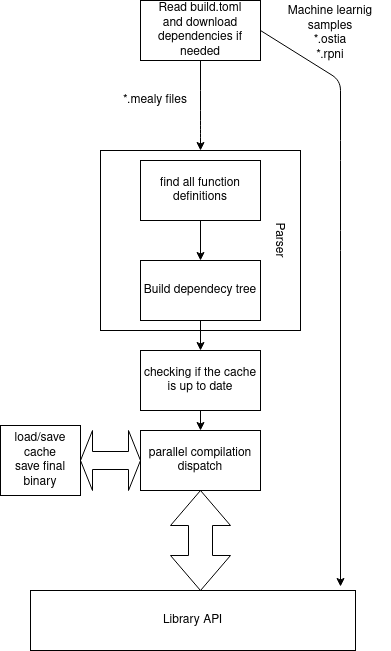
\includegraphics{./diagram.png}
\caption{Build process}
\label{buildsystem:diagram}
\end{figure}

\hypertarget{parsing-sources}{%
\subsubsection{Parsing sources}\label{dependency-resolving}}

Before starting the compilation, it is necessary to find a list of all
function definitions at the beginning, which will then allow the cache
to be loaded and the dependency graph to be mapped to make the process
convenient and efficient. To do this it is necessary to pre-parse all
source files. 
For this purpose, we use ANTLR and the grammar identical to that used
in the library. However, the parser itself is very simplified. It works
down to writing down the names of functions, their types and their bodies. 

\hypertarget{dependency-resolving}{%
\subsubsection{Dependency resolving}\label{dependency-resolving}}

The problem is that function definitions can be located in different
files on any position and functions can be nested (one function can be
used in a body of another one). Before starting the compilation, it is
worth checking immediately whether it has a chance to succeed at all. To
accomplish this, Solomonoff first loads code from repositories and
user-supplied source code, and then parses it. ANTLR was used to
generate the parser. During the process a directed acyclic graph is
generated. The graph represents relations of being a dependency of a
another node which represent functions. The system uses JGraphT to
create this graph and to sort it topologically. This sorting algorithm
guarantees that if we start compiling functions in order that sorting
function returned us the necessary dependencies for each subsequent
element will already be compiled.

Topological sort is based on the Kahn's algorithm.

In the constructor fragment cited below, a list of source nodes is
created.

\begin{lstlisting}[language=Java, frame=single]
...
this.inDegreeMap = new HashMap<>();
for (V v : graph.vertexSet()) {
    int d = 0;
    for (E e : graph.incomingEdgesOf(v)) {
        V u = Graphs.getOppositeVertex(graph, e, v);
        if (v.equals(u)) {
            throw new IllegalArgumentException(GRAPH_IS_NOT_A_DAG);
        }
        d++;
    }
    inDegreeMap.put(v, new ModifiableInteger(d));
    if (d == 0) {
        queue.offer(v);
    }
}

this.remainingVertices = graph.vertexSet().size();
...
\end{lstlisting}

The advance method called, for each iteration, will initially return the
existing sources nodes and then the new ones which appears after
removing the previous ones, and so on to the last vertex.

\begin{lstlisting}[language=Java, frame=single]
private V advance()
{
    V result = queue.poll();

    if (result != null) {
        for (E e : graph.outgoingEdgesOf(result)) {
            V other = Graphs.getOppositeVertex(graph, e, result);

            ModifiableInteger inDegree = inDegreeMap.get(other);
            if (inDegree.value > 0) {
                inDegree.value--;

                if (inDegree.value == 0) {
                    queue.offer(other);
                }
            }
        }

        --remainingVertices;
    } else {
        /*
         * Still expecting some vertices, but no vertex has zero degree.
         */
        if (remainingVertices > 0) {
            throw new IllegalArgumentException(GRAPH_IS_NOT_A_DAG);
        }
    }

    return result;
}
\end{lstlisting}

\hypertarget{parallel-building}{%
\subsubsection{Parallel building}\label{parallel-building}}

The next step is compilation. To achieve compilation efficiency, the
functions are put in the mentioned order in the queue from which they
will be then downloaded to the Thread pool, if the compilation of their
dependencies has already finished. In this way, we are to use the full
potential of the CPU that the operating system will make available to
us.

The code below shows how the parallel compilation problem is solved.

\begin{lstlisting}[language=Java, frame=single]
...
// already sorted dependencies
while (dependencyOrder.hasNext()) {

    final String id = dependencyOrder.next();
    final VarDef<G> varDef = definitions.get(id);

    if (varDef == null) {//This may only be true for built-in variables
        assert compiler.specs.borrowVariable(id) != null : id;

    } else if (varDef instanceof VarDefAST) {
        VarDefAST<G> var = (VarDefAST<G>) varDef;
        assert var.def != null : id;

        compiled.put(id, pool.submit(() -> {
            if (var.needsRecompilation) {
                final G compiledGraph = var.def.compile(compiler.specs, i -> {
                    try {
                        final Future<G> f = compiled.get(i);
                        if (f == null) {//this can only be true for built-in variables
                            final LexUnicodeSpecification.Var<N, G> v = compiler.specs.copyVariable(i);
                            assert v != null;
                            final G graph = compiler.specs.getGraph(v);
                            return graph;
                        } else {
                            final G graph = compiler.specs.deepClone(f.get());
                            return graph;
                        }
                    } catch (InterruptedException | ExecutionException e) {
                        throw new RuntimeException(e);
                    }
                });

                System.err.println("Compiled " + id);

                if (buildBin) {
                    try (FileOutputStream f = new FileOutputStream(var.cacheFilePath.toFile())) {
                        compiler.specs.compressBinary(compiledGraph, new DataOutputStream(f));
                    } catch (IOException e) {
                        e.printStackTrace();
                        var.cacheFilePath.toFile().deleteOnExit();
                    }
                }
                return compiledGraph;
            } else {
                System.err.println("Loaded from cache " + id);
                try (DataInputStream dis =
                             new DataInputStream(new FileInputStream(var.cacheFilePath.toFile()))) {
                    return compiler.specs.decompressBinary(Pos.NONE, dis);
                }
            }
        }));
    }
}
...
\end{lstlisting}

\hypertarget{caching-transducers}{%
\subsubsection{Caching transducers}\label{caching-transducers}}

To achieve this goal, an analogous mechanism was used to that used in
GNU Make. When parsing the code, we retrieve information about the
modification date of a given source from the file system. If the user
did not order otherwise, before the compilation starts, the modification
dates of previously compiled transducers saved on the disk will be read
and then both will be quickly compared. If the binary file date is not
older than the source code date and the same situation repeats for all
dependencies of the given function, it will not be compiled again at
this point.

The code below shows how to check if the compiled transducer is
up-to-date with the source code.

\begin{lstlisting}[language=Java, frame=single]
protected VarDef(String id, String sourceFile, Config config) throws IOException {
    ...
    if (sourceFile == null) {
        this.needsRecompilation = false;
        return;
    }
    final Path sourceFilePath = Paths.get(sourceFile);
    final FileTime sourceFileModificationTime =
            (FileTime) Files.getAttribute(sourceFilePath, "lastModifiedTime");
    final boolean needsRecompilation;
    if (!config.caching_read && config.caching_write) {
        needsRecompilation = true;
    } else if (Files.exists(cacheFilePath)) {
        final FileTime cacheModificationTime =
                (FileTime) Files.getAttribute(cacheFilePath, "lastModifiedTime");
        final int diff = cacheModificationTime.compareTo(sourceFileModificationTime);
        needsRecompilation = diff < 0;
    } else {
        needsRecompilation = true;
    }
    this.needsRecompilation = needsRecompilation;
}
\end{lstlisting}

Here we go through the dependency tree to check if any of the
dependencies out of date will force a cascading recompilation. 

\begin{lstlisting}[language=Java, frame=single]
...
//Resolve which dependencies need to be recompiled
final Stack<VarDef<G>> toCheckIfNeedsRecompilation = new Stack<>();
for (VarDef<G> def : definitions.values()) {
    if (!def.needsRecompilation) {
        toCheckIfNeedsRecompilation.add(def);
    }
}
while (!toCheckIfNeedsRecompilation.isEmpty()) {
    final VarDef<G> definition = toCheckIfNeedsRecompilation.pop();
    assert !definition.needsRecompilation;
    boolean actuallyShouldBeRecompiled = false;
    for (Object dependencyEdge : dependencyOf.incomingEdgesOf(definition.id)) {
        final String dependencyOfVertex = dependencyOf.getEdgeSource(dependencyEdge);
        final VarDef<G> definitionOfDependency = definitions.get(dependencyOfVertex);
        if (definitionOfDependency != null/*built-in variables don't need to recompiled*/
                && definitionOfDependency.needsRecompilation) {
            actuallyShouldBeRecompiled = true;
            break;
        }
    }
    if (actuallyShouldBeRecompiled) {
        definition.needsRecompilation = true;
        for (Object dependedEdge : dependencyOf.outgoingEdgesOf(definition.id)) {
            final String idToReconsider = dependencyOf.getEdgeTarget(dependedEdge);
            final VarDef<G> definitionToReconsider = definitions.get(idToReconsider);
            if (!toCheckIfNeedsRecompilation.contains(definitionToReconsider)) {
                toCheckIfNeedsRecompilation.add(definitionToReconsider);
            }
        }
    }
}
...
\end{lstlisting}

\hypertarget{setting-up-form-a-file}{%
\subsubsection{Setting up form a file}\label{setting-up-form-a-file}}

Build.toml file which delivers a configuration to the build system
describes the project metadata, contains the program's configurations
such as repository paths, and defines the sources from which the system
loads the code for compilation. An example file is shown below.

\begin{verbatim}
project_name = "test" # project name (needed during export)
version = 1.0 # project version (needed during export)
private_key  = "./private.der" 
# private key (needed during export until sign_pkg equals false) 
# RSA with SHA256 'der' format
sign_pkg = true

cache_location = "bin/" # bin is default 
#local_repo = "" # custom location (default is $USER_HOME/.Solomonoff)

[[source]]
path = "sample3.mealy"

[[source]]
path = "sample4.ostia"

[[pkg]]
public_key  = "pubkey.der" # publickey RSA with SHA256 'der' format
name = "test" 
version = "1.0"
remote_repo = "https://solomonoff.projektstudencki.pl/repo/"
verify_signature = true
\end{verbatim}

The system uses TOML markup language as it gives us the greatest
flexibility.

\hypertarget{package-manager}{%
\subsubsection{Package manager}\label{package-manager}}

Solomonoff comes with a very simplified package manager. To download a
package, the build system, using HTTP or HTTPS, queries the remote
repository for the requested package and downloads it to the local
repository if it is available. Also, the signature is downloaded if the
user has not requested otherwise. If the user tries to download the same
package again in the same version, it will not be downloaded since it is
already in the local repository. For this reason, the naming convention
is very important. Our suggestion is to keep project names as
\texttt{\textless{}developer\_email@example.com\textgreater{}\ \textless{}desired\_project\_name\textgreater{}}
in order to avoid a collision. Packages and signatures have names in the
following format
\texttt{\textless{}project\_name\textgreater{}\ -\ \textless{}version\textgreater{}\ .zip\ {[}.sig{]}}.
This very simple system allows you to use any web server as a remote
repository without the need to install special software. 

Package manager can also export a package. The package is a pair of zip archive
and its signature. The archive only contains the code, because
compilation does not take so long that it makes sense to distribute
already compiled automatons.
